% ------------------------------------------------------------------------------
% TYPO3 CMS 7.6 - What's New - Chapter "Introduction" (English Version)
%
% @author	Michael Schams <schams.net>
% @license	Creative Commons BY-NC-SA 3.0
% @link		http://typo3.org/download/release-notes/whats-new/
% @language	English
% ------------------------------------------------------------------------------
% LTXE-CHAPTER-UID:		cb43d098-7bf9a537-bf3817c0-53a0f29f
% LTXE-CHAPTER-NAME:	Introduction
% ------------------------------------------------------------------------------

\section{Inleiding}
\begin{frame}[fragile]
	\frametitle{Inleiding}

	\begin{center}\huge{Inleiding}\end{center}
	\begin{center}\huge{\color{typo3darkgrey}\textbf{De feiten}}\end{center}

\end{frame}

% ------------------------------------------------------------------------------
% LTXE-SLIDE-START
% LTXE-SLIDE-UID:		aeee51b6-fa5cfb5f-4444db3c-1d303916
% LTXE-SLIDE-ORIGIN:	9e397afb-762f7061-0e0e0bd1-9836250e English
% LTXE-SLIDE-ORIGIN:	1e50fa0a-e0f4c00a-5f667356-11df7c7c German
% LTXE-SLIDE-TITLE:		TYPO3 CMS 7.6 - The Facts
% ------------------------------------------------------------------------------
\begin{frame}[fragile]
	\frametitle{Inleiding}
	\framesubtitle{TYPO3 CMS 7.6 - De feiten}

	\begin{itemize}
		\item Publicatiedatum: 10 november 2015
		\item Publicatietype:
			\begingroup\color{red}Long Term Support (LTS) Publicatie\endgroup
		\item Visie: Omarm, Innoveer, Verspreid
	\end{itemize}

	\begin{figure}
		
\includegraphics[width=0.95\linewidth]{Introduction/typo3cms76-banner.png}
	\end{figure}

\end{frame}

% ------------------------------------------------------------------------------
% LTXE-SLIDE-START
% LTXE-SLIDE-UID:		3507b8a4-509e568d-7441aa0a-a45fb959
% LTXE-SLIDE-ORIGIN:	737c8e9b-4ae60e26-6975ea72-21146dd0 English
% LTXE-SLIDE-ORIGIN:	07f94e22-95cf3db6-373b81e0-4b00bb57 German
% LTXE-SLIDE-TITLE:		System Requirements
% ------------------------------------------------------------------------------
\begin{frame}[fragile]
	\frametitle{Inleiding}
	\framesubtitle{Systeemeisen}

	\begin{itemize}
		\item PHP*:\tabto{2.2cm}v5.5.0 - v5.6.x
		\item MySQL:\tabto{2.2cm}v5.5.x - v5.6.x (geen strict mode)
		\item Schijfruimte:\tabto{2.2cm}min 200 MB
		\item PHP-instellingen:

			\begin{itemize}
				\item memory\_limit >= 128M
				\item max\_execution\_time >= 240s
				\item compilatie optie \texttt{-}\texttt{-disable-ipv6} \underline{niet} gebruiken
			\end{itemize}

		\item Backend vereist IE >= 9 of een andere moderne browser

	\end{itemize}

	\vspace{1cm}

	*) Meer details: \href{http://typo3.org/news/article/php-minimum-requirements-for-typo3-cms-7/}{PHP Minimum Requirements for TYPO3 CMS 7}

\end{frame}

% ------------------------------------------------------------------------------
% LTXE-SLIDE-START
% LTXE-SLIDE-UID:		c740c8f6-1213211e-48abfa32-14574e7b
% LTXE-SLIDE-ORIGIN:	90d2d3d1-f9d57661-dd01143b-10630416 English
% LTXE-SLIDE-ORIGIN:	79b3ee12-a96f5128-178eb0a1-52534b81 German
% LTXE-SLIDE-TITLE:		Development And Release Timeline
% ------------------------------------------------------------------------------
\begin{frame}[fragile]
	\frametitle{Inleiding}
	\framesubtitle{Ontwikkelings- en publicatietijdlijn}

	\begin{figure}
		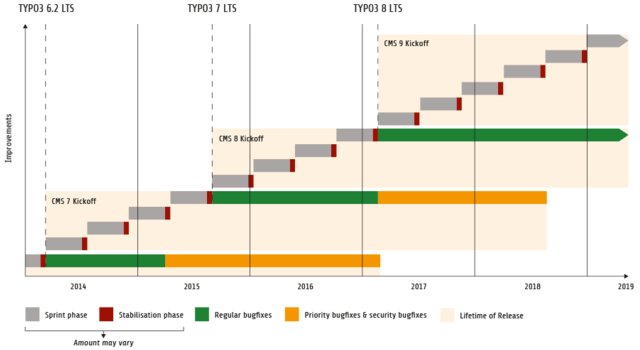
\includegraphics[width=0.90\linewidth]{Introduction/ReleaseAgenda.png}
	\end{figure}

\end{frame}

% ------------------------------------------------------------------------------
% LTXE-SLIDE-START
% LTXE-SLIDE-UID:		dc9a6970-12a63b21-9b6c6e5b-954b39d9
% LTXE-SLIDE-ORIGIN:	13e0fd6a-fa50d02d-c15c4af0-f3996926 English
% LTXE-SLIDE-ORIGIN:	89509115-eb2b6501-4bf03801-c53e7c0c German
% LTXE-SLIDE-TITLE:		TYPO3 CMS Roadmap
% ------------------------------------------------------------------------------
\begin{frame}[fragile]
	\frametitle{Inleiding}
	\framesubtitle{TYPO3 CMS Roadmap}

	Geschatte publicatiedatum en primaire focus:

	\begin{itemize}
		\item v7.0 \tabto{1.1cm}02 dec 2014\tabto{3.4cm}Backend makeover deel 1
		\item v7.1 \tabto{1.1cm}24 feb 2015\tabto{3.4cm}Core opschonen en stroomlijnen
		\item v7.2 \tabto{1.1cm}28 apr 2015\tabto{3.4cm}Frontend
		\item v7.3 \tabto{1.1cm}16 jun 2015\tabto{3.4cm}Package Ecosysteem, Composer
		\item v7.4 \tabto{1.1cm}04 aug 2015\tabto{3.4cm}Backend makeover deel 2
		\item v7.5 \tabto{1.1cm}29 sep 2015\tabto{3.4cm}Afronding

		\item
			\begingroup
				\color{typo3orange}
					v7 LTS \tabto{1.1cm}10 nov 2015\tabto{3.4cm}\textbf{TYPO3 CMS 7 LTS} (Long Term Support)
			\endgroup

	\end{itemize}

	\smaller
		\url{https://typo3.org/typo3-cms/roadmap/}\newline
		\url{http://typo3.org/news/article/embrace-and-innovate-typo3-cms-7/}
	\normalsize

\end{frame}

% ------------------------------------------------------------------------------
% LTXE-SLIDE-START
% LTXE-SLIDE-UID:		3eda60ba-bb8f4849-ce10917b-540bd0b4
% LTXE-SLIDE-ORIGIN:	06c6100a-69216610-618bde63-bbdc4eef English
% LTXE-SLIDE-ORIGIN:	8ac7908b-f1a64895-d12d437b-9309b07b German
% LTXE-SLIDE-TITLE:		Installation
% ------------------------------------------------------------------------------
\begin{frame}[fragile]
	\frametitle{Inleiding}
	\framesubtitle{Installatie}

	\begin{itemize}
		\item Officiële installatieprocedure op Linux/Mac OS X\newline
			(DocumentRoot bijvoorbeeld \texttt{/var/www/site/htdocs}):
		\begin{lstlisting}
			$ cd /var/www/site
			$ wget --content-disposition get.typo3.org/7.6
			$ tar xzf typo3_src-7.6.0.tar.gz
			$ cd htdocs
			$ ln -s ../typo3_src-7.6.0 typo3_src
			$ ln -s typo3_src/index.php
			$ ln -s typo3_src/typo3
			$ touch FIRST_INSTALL
		\end{lstlisting}

		\item Symbolische koppelingen op Microsoft Windows:

			\begin{itemize}
				\item Gebruik \texttt{junction} met Windows XP/2000
				\item Gebruik \texttt{mklink} met Windows Vista en Windows 7
			\end{itemize}

	\end{itemize}
\end{frame}

% ------------------------------------------------------------------------------
% LTXE-SLIDE-START
% LTXE-SLIDE-UID:		423ab2b9-58dd0f54-d520cce2-cfb7982e
% LTXE-SLIDE-ORIGIN:	e4b09ddf-4c0ea575-9e0900ad-b878899c English
% LTXE-SLIDE-ORIGIN:	d146f854-4fcfed01-7de68fce-c2599f7f German
% LTXE-SLIDE-TITLE:		Upgrade to TYPO3 CMS 7
% ------------------------------------------------------------------------------
\begin{frame}[fragile]
	\frametitle{Inleiding}
	\framesubtitle{Upgrade naar TYPO3 CMS 7.x}

	\begin{itemize}
		\item Upgrades alleen mogelijk van TYPO3 CMS 6.2 LTS
		\item TYPO3 CMS < 6.2 moet eerst worden geüpgrade naar TYPO3 CMS 6.2 LTS
	\end{itemize}

	\begin{itemize}

		\item Upgrade-instructies:\newline
			\smaller\url{http://wiki.typo3.org/Upgrade#Upgrading_to_7.6}\normalsize
		\item Officiële TYPO3-handleiding "TYPO3 Installation and Upgrading":
			\smaller\url{http://docs.typo3.org/typo3cms/InstallationGuide}\normalsize
		\item Algemene aanpak:
			\begin{itemize}
				\item Controleer minimale systeemeisen (PHP, MySQL, etc.)
				\item Inspecteer \textbf{deprecation\_*.log} in oude TYPO3-installatie
				\item Werk alle extensies bij naar de nieuwste versie
				\item Zet nieuwe bronbestanden neer en start\newline
					Installatie-module \textrightarrow Upgrade Wizard
				\item Check startmodule voor backend gebruikers (optioneel)
			\end{itemize}
	\end{itemize}

\end{frame}

% ------------------------------------------------------------------------------
